% !TEX root = ../meca1321-synthesis.tex

\chapter{Couches limites laminaires}
  \section{Introduction}
    Malgré son utilité, le modèle du fluide parfait en écoulement incompressible et irrotationnel est limité aux écoulements avec glissement de fluides le long des parois, ce qui n'est pas le comportement des fluides réels qui y adhèrent. Cette adhérence génère du tourbillon le long de la paroi. Le fluide n'y est donc plus irrotationnel. La zone proche de la paroi contenant ce tourbillon est appelée ``couche limite (de paroi)''.

    Son épaisseur est déterminée par la compétition entre diffusion et convection du tourbillon et est généralement mince, s'amincissant avec l'augmentation du Reynolds.

    Soit un écoulement laminaire autour d'un profil de type aérodynamique à faible angle d'attaque. La vitesse caractéristique est la vitesse en amont $U_\infty$ et la dimension caractéristique globale est la corde du profil $c$. Le Reynolds est donc $Re_c = U_\infty c / \nu$ et le temps caractéristique global de convection est $T \propto c/U_\infty$\footnote{Il s'agit du temps requis pour qu'une particule aille du bord d'attaque du profil jusqu'au bord de fuite.}. Au sein de la couche limite, les effets de la viscosité sont du même ordre de grandeur que les effets d'inertie\footnote{Il s'agit aussi d'une définition alternative de la couche limite}. Dans ce cas ici considéré, le temps $T$ est aussi le temps caractéristique global de diffusion du tourbillon dans de la couche limite. Durant ce temps, la diffusion va avoir couvert une épaisseur globale $\delta \propto \sqrt{\nu T}$. Ainsi
    \begin{equation}
      T \propto \frac{\delta^2}{\nu} \quad \textrm{et} \quad T \propto \frac{c}{U_\infty}
    \end{equation}
    ce qui conduit à
    \begin{equation}
      \begin{aligned}
        \delta^2 &\propto \nu T \propto \frac{\nu c}{U_\infty} = \frac{c^2}{\frac{U_\infty c}{\nu}}\\
        \frac{\delta}{c} &\propto \recip{\sqrt{\frac{U_\infty c}{\nu}}} = \recip{\sqrt{Re_c}}
      \end{aligned}
    \end{equation}

    Dans les expressions ci-dessus, $\delta$ désigne l'épaisseur de la couche limite au bord au bord de fuite du profil (\textit{i.e.} en $x=c$). À une distance $x < c$ le long du profil, on obtient alors
    \begin{equation}
      \begin{aligned}
        \delta^2(x) &\propto \frac{\nu c}{U_\infty} f\left(\frac{x}{c}\right) = \frac{c^2}{\frac{U_\infty c}{\nu}}f\left(\frac{x}{c}\right)\\
        \frac{\delta(x)}{c} &\propto \recip{\sqrt{Re_c}} \sqrt{f\left(\frac{x}{c}\right)}
      \end{aligned}
    \end{equation}

    En aval du profil, la couche limite devient tourbillon de sillage, cas idéal de bon fonctionnement du profil. En réalité, la couchle limite à l'extrados aura tendance à quitter la paroi avant d'atteindre le bord de fuite. On parle de ``séparation de la couche limite''. Celle-ci mène à une baisse de performance du profil (\textit{i.e.} une baisse de portance) mais sans être catastrophique. Cependant, si on augmente l'angle d'attaque, on aura un ``décrochage aérodynamique'', cas de mauvais fonctionnement aérodynamique. Le tourbillon quitte alors brutalement la paroi et des tourbillons de sillages sont produits de façon intermittente, le point de séparation étant instationnaire.

    Ce chapitre expose la théorie de la ``couche limite laminaire'' pour des écoulements simples et incompressibles. On considère une couche limite le long d'une plaque plane avec vitesse hors couche limite $u_e = u_e(x)$. On obtiendra ensuite le cas avec $u_e$ constant (solution de Blasius).

  \section{Établissement des équations de la couche limite laminaire}
    \subsection{Approche physique, non formelle}
      Soit un écoulement laminaire bidimensionnel et stationnaire le long d'une plaque plane. La plaque et la couche limite commencent en $x=0$.

      Sans couche limite, on a une vitesse d'écoulement connue\footnote{Par exemple, calculée via l'approximation du fluide parfait.}. On suppose la couche limite assez mince pour que la vitesse en dehors $u_e(x)$ soit approximable par la vitesse obtenue sans couche limite. Au sein de la couche limite, la valeur passe de $0$ à la paroi à $u_e(x)$.

      Via l'introduction, l'épaisseur de la couche limite $\delta(x=X)$ est faible par rapport à $X$ ($\delta \ll X$). $\pdv{u}{y}$ est donc $\mathcal{O}(U_e/\delta)$ et $\pdv{u}{x}$ est $\mathcal{O}(U_e/X)$. On a donc
      \begin{equation}\label{eq:diffvisq}
        \begin{aligned}
          \left| \pdv{u}{x} \right| = \mathcal{O}\left(\frac{U_e}{X}\right) &\ll \left|\pdv{u}{y}\right| = \mathcal{O}\left(\frac{U_e}{\delta}\right)\\
          \left| \pdv[2]{u}{x} \right| = \mathcal{O}\left(\frac{U_e}{X^2}\right) &\ll \left|\pdv[2]{u}{y}\right| = \mathcal{O}\left(\frac{U_e}{\delta^2}\right)
        \end{aligned}
      \end{equation}

      Soit $V$ l'ordre de grandeur de la vitesse verticale $v$ dans la couche limite $v = \mathcal{O}(V)$. Ainsi
      \begin{equation}
        \left|\pdv{v}{y}\right| = \mathcal{O}\left(\frac{V}{\delta}\right)
      \end{equation}
      L'équation de continuité $\pdv{u}{x} + \pdv{v}{y} = 0$ implique aussi
      \begin{equation}
        \begin{aligned}
          \left|\pdv{v}{y}\right| &\sim \left| \pdv{u}{x} \right| = \mathcal{O} \left(\frac{U_e}{X}\right)\\
          \left|\pdv{v}{y}\right| &= \mathcal{O} \left(\frac{V}{\delta}\right) = \mathcal{O} \left(\frac{U_e}{X}\right)\\
          V &= \frac{\delta}{X} U_e
        \end{aligned}
      \end{equation}

      L'équation de quantité de mouveemnt dans la direction horizontale $x$ est alors
      \begin{equation}
        u\pdv{u}{x} + v\pdv{u}{y} = -\recip{\rho} \pdv{p}{x} + \nu \left(\pdv[2]{u}{x} + \pdv[2]{u}{y}\right)
      \end{equation}
      Les ordres de grandeurs des termes d'inertie sont
      \begin{equation}
        \left|u \pdv{u}{x} \right| = \mathcal{O}\left(\frac{U_e^2}{X}\right), \quad \left|v\pdv{u}{y}\right| \mathcal{O}\left(\frac{\delta}{X} U_e \frac{U_e}{\delta}\right) = \mathcal{O}\left(\frac{U_e^2}{X}\right)
      \end{equation}
      Les termes de diffusion visqueuse sont tels qu'ils sont négligeables en $x$ par rapport à $y$, par \ref{eq:diffvisq}. On considère donc
      \begin{equation}
        \left|\nu \pdv[2]{u}{y}\right| = \mathcal{O}\left(\nu \frac{U_e}{\delta^2}\right)
      \end{equation}

      La couche limite étant la zone où les effets de viscosités sont aussi importants que les effets d'inertie, on a
      \begin{equation}
        \begin{aligned}
          \left|u\pdv{u}{x}\right| \sim \left|v \pdv{u}{y} \right| \sim \left|\nu \pdv[2]{u}{y} \right| = \mathcal{O}\left(\frac{U_e^2}{X}\right)\\
          \delta^2 = \frac{\nu X}{U_e} \quad \Rightarrow \quad \frac{\delta}{X} = \left(\frac{U_e X}{\nu}\right)^{-\frac{1}{2}}
        \end{aligned}
      \end{equation}
      qui est le résultat de l'introduction.

      Comme le terme $\recip{\rho} \left|\pdv{p}{x}\right|$ est un des termes de l'équation de mouvement, il est soit négligeable soit $\mathcal{O}(U_e^2/X)$. Au delà de $\delta$, l'écoulement est irrotationnel: Bernoulli est satisfait
      \begin{equation}
        \begin{aligned}
          \frac{p_e(x)}{\rho} + \frac{u_e^2(x)}{2} = B_0\\
          -\recip{rho} \pdv{p_e}{x}(x) = u_e(x) \pdv{u_e}{x}(x)
        \end{aligned}
      \end{equation}

      Considérons désormais l'équation dans la direction verticale $y$
      \begin{equation}
        u\pdv{v}{x} + v \pdv{v}{y} = -\recip{\rho}\pdv{p}{y} + \nu \left(\pdv[2]{v}{x} + \pdv[2]{v}{y}\right)
      \end{equation}
      Les termes d'inerties sont d'ordre de grandeur
      \begin{equation}
        \left|u \pdv{v}{x} \right| \sim \left|v\pdv{v}{y}\right| \sim \mathcal{O}\left(U_e \frac{V}{X} \right) =
        \mathcal{O}\left(\frac{V^2}{\delta}\right) = \mathcal{O}\left(\frac{\delta}{X}\frac{U_e^2}{X}\right)\\
      \end{equation}
      La diffusion est négligeable en $x$ par rapport à $y$
      \begin{equation}
        \left| \nu \pdv[2]{v}{y} \right| = \mathcal{O}\left(\nu \frac{V}{\delta}\right) = \mathcal{O}\left(\nu \frac{\delta}{X}\frac{U_e}{\delta^2}\right)
      \end{equation}
      Le terme de pression est donc aussi, au plus, de cet ordre de grandeur. Par série de Taylor, la pression est donc
      \begin{equation}
        p(x, y) = p_e(x) + (y-\delta) \pdv{p}{y}\eval_{y_\delta} + ...
      \end{equation}
      ce qui donne
      \begin{equation}
        \begin{aligned}
          \frac{p(x,y)}{\rho} = \frac{p_e(x)}{\rho} + \mathcal{O}\left(\delta \frac{\delta}{X}\frac{U_e^2}{X}\right) &= \frac{p_e(x)}{\rho} + \mathcal{O}\left(\left(\frac{\delta}{X}\right)^2 U_e^2\right)\\
          &= B_0 - \left(1 - \mathcal{O}\left(\left(\frac{\delta}{X}\right)^2\right)\right) \frac{u_e^2(x)}{2}
        \end{aligned}
      \end{equation}
      Le terme de correction étant en $(\delta/X)^2$, on peut le négliger et considérer la pression constante au travers de la couche limite. On a donc $p(x, y) = p_e(x)$, soit
      \begin{equation}
        -\recip{\rho} \pdv{p}{x} = -\recip{\rho}\dv{p_e}{x}(x) = u_e(x) \dv{u_e}{x}(x)
      \end{equation}
      Les équations régissant le développement de la couche limite, dites ``de Prandtl'' sont donc
      \begin{equation}
        \begin{aligned}
          \pdv{u}{x} + \pdv{v}{y} &= 0\\
          u \pdv{u}{x} + v \pdv{u}{y} &= u_e \dv{u_e}{x} + \nu \pdv[2]{u}{y}
        \end{aligned}
      \end{equation}

    \subsection{Approche formelle mathématique}
      La couche se développe sur une plaque plane commençant en $x=0$. On évalue la couche limite autour de $X$ avec une vitesse extérieure $U_e = u_e(X)$. Il y a donc deux ``grandeurs caractéristiques'' constantes. Le nombre de Reynolds est donc $Re = U_eX/\nu$. Pour voir comment l'écoulement se comporte pour $Re$ grand, on adimensionnalise les équations en $X$ et $U_e$ et on prend $Re \rightarrow \infty$.

      Soit une famille d'écoulements fictifs, paramétrés par $Re$ qu'on fait tendre vers l'infini (similitude dynamique). L'écoulement asymptotique obtenu par passage à la limite est une bonne approximation de l'écoulement réel, correspondant à une valeur précise de $Re$. La comparaison de ces écoulements n'est possible qu'en adimensionnalisant les équations.

      La première adimensionnalisation fait apparaître les équations d'Euler pour $Re \rightarrow \infty$ . Il s'agit de l'écoulement ``externe'' du fluide parfait ne respectant pas les conditions sur la plaque. Une seconde adimensionnalisation fait apparaître la couche limite et les équations de Prandtl.

      Soit $\delta = Re^{-1/2} X$, l'ordre de grandeur de l'épaisseur de la couche limite en $X$. Soit la mise sous forme adimensionnelle en utilisant les variables ``prime'' adimensionnelles suivantes
      \begin{equation}
        x = x'X, \quad u=y' \delta, \quad u = u'U_e, \quad v = v' V, \quad \textrm{et} \quad p = p' \rho U_e^2
      \end{equation}
      où $V$ est à déterminer. L'équation de continuité devient alors
      \begin{equation}
        \begin{aligned}
          \frac{U_e}{X} \pdv{u'}{x'} + \frac{V}{\delta} \pdv{v'}{y'} &= 0\\
          \pdv{u'}{x'} = -\frac{V}{U_e} \frac{X}{\delta}\pdv{v'}{y'} = -\frac{V}{U_e}Re^{\frac{1}{2}}\pdv{v'}{y'}
        \end{aligned}
      \end{equation}
      Pour que l'équation ne dégénère pas en $Re \rightarrow \infty$ (principe de dégénérescence), on doit prendre
      \begin{equation}
        V  = \frac{U_e}{Re^{\frac{1}{2}}}
      \end{equation}
      et donc
      \begin{equation}
        \pdv{u'}{x'} + \pdv{v'}{y'} = 0
      \end{equation}
      L'équation de la quantité de mouvement en $x$ donne
      \begin{equation}
        \begin{aligned}
          \frac{U_e^2}{X} \left(u' \pdv{u'}{x'} + v' \pdv{u}{y'}\right) &= - \frac{U_e^2}{X}\pdv{p'}{x'} + \frac{\nu U_e}{X^2}\prpdv{u}{x} + \frac{\nu U_e}{\delta^2} \prpdv{u}{y}\\
          &= - \frac{U_e}{X}\pdv{p'}{x'} + \frac{\nu U_e}{\delta^2} \left(\left(\frac{\delta}{X}\right)^2 \prpdv{u}{x} + \prpdv{u}{y}\right)\\
          &= - \frac{U_e^2}{X}\pdv{p'}{x'} + \frac{U_e^2}{X} \left(\recip{Re}\prpdv{u}{x} + \pdv{u}{y}\right)
        \end{aligned}
      \end{equation}
      Par conséquent,
      \begin{equation}
        u'\pdv{u'}{x'} + v'\pdv{u'}{y'} = -\pdv{p'}{x'} + \left(\recip{Re} \prpdv{u}{x} + \prpdv{u}{y}\right)
      \end{equation}
      et, en $Re \rightarrow \infty$
      \begin{equation}
        u'\pdv{u'}{x'} + v'\pdv{u'}{y'} = -\pdv{p'}{x'} + \prpdv{u}{y}
      \end{equation}

      En $y$, on obtient
      \begin{equation}
        \begin{aligned}
          \frac{U_e V}{X} \left(u' \pdv{v'}{x'} + v' \pdv{v'}{y'}\right) &= - \frac{U_e^2}{\delta}\pdv{p'}{y'} + \nu \frac{V}{\delta^2} \left(\left(\frac{\delta}{X}\right)^2 \prpdv{v}{x} + \prpdv{v}{y} \right)\\
          \recip{Re} \left(u' \pdv{u'}{x'} + v'\pdv{v'}{y'}\right) &= -\pdv{p'}{y'} + \recip{Re} \left(\recip{Re}\prpdv{v}{x} + \prpdv{v}{y}\right)\\
          \pdv{p'}{y'} &= 0 \quad \quad \textrm{en } Re \rightarrow \infty
        \end{aligned}
      \end{equation}
      La pression ne varie donc pas dans la couche limite. Les conditions à la paroi sont $u = v = 0$ tandis que les conditions à distance de la paroi sont le raccord entre les écoulements de Prandtl et d'Euler. Soit $\zeta = Re^{-1/4} X$. Comme $Re \gg 1$, on a
      \begin{equation}
        \frac{\delta}{\zeta} = \recip{Re^{1/4}} \ll 1 \quad \textrm{et} \quad \frac{\zeta}{X} = \recip{Re^{1/4}} \ll 1 \quad \Rightarrow \quad \delta \ll \zeta \ll X
      \end{equation}
      On considère que le raccordement Prandtl-Euler se fait à hauteur $\mathcal{O}(\zeta)$. Pour les valeurs de $Re$ grandes, la solution adimmensionnelle a une valeur unique au raccordement. Cependant, l'ordonnée adimensionnelle de raccordement est $\hat{y} = \zeta/X \ll 1$ pour la zone externe et $\tilde{y} = \zeta/\delta \ll 1$ pour la zone interne. En faisant tendre $Re$ vers l'infini, on a une ordonnée tendant vers $0$ pour la couche externe  et vers l'infini pour la zone interne.

      On a donc comme conditions asymptotique de raccordement
      \begin{equation}
        \begin{aligned}
          \lim_{y/\delta \gg 1} u(X, y) &= \lim_{y/X \ll 1} u_e(X, y) = u_e(X, 0) = U_e\\
          \lim_{y/\delta \gg 1} p(X, y) &= \lim_{y/X \ll 1} p_e(X, y) = p_e(X, U)
        \end{aligned}
      \end{equation}
      \begin{multicols}{2}
        \begin{equation*}
          \begin{aligned}
            \pdv{u}{x} + \pdv{v}{y} &= 0\\
            u \pdv{u}{x} + v\pdv{u}{y} &= \underbrace{-\recip{\rho}{\pdv{p_e}{x}}(x, 0)}_{=u_e(x, 0){\pdv{u_e}{x}}(x,0)} + \nu\pdv[2]{u}{y}
          \end{aligned}
        \end{equation*}

        \begin{equation}
          \begin{aligned}
            u(x, 0) &= v(x, 0) = 0\\
            \lim_{y/\delta \gg 1} u(x, y) &= u_e(x, 0)
          \end{aligned}
        \end{equation}
      \end{multicols}

  \section{Solution pour le cas avec $u_e$ constant (Blasius)}
    \begin{equation}
      \begin{aligned}
        \pdv{u}{x} + \pdv{u}{y} &= 0\\
        u\pdv{u}{x} + v \pdv{u}{y} &= \nu \pdv[2]{u}{y}
      \end{aligned}
    \end{equation}
    Le champ de vitesse de l'écoulement incompressible est une fonction de courant $\psi : u = \pdv*{\psi}{y}$ et $v = - \pdv*{\psi}{x}$. La similitude de la solution requiert que
    \begin{equation}
      \frac{u}{u_e} = g\left(\frac{y}{\delta(x)}\right) = g(\eta)
    \end{equation}
    où $\eta = u/\delta(x)$ est la variable de similitude où\footnote{Le facteur $2^{1/2}$ n'est pas nécessaire mais permet d'éviter un facteur 2 plus loin}
    \begin{equation}
      \delta(x) = \frac{x}{\left(\frac{u_e x}{2\nu}^{1/2}\right)} = \frac{2^{1/2}x}{Re^{1/2}} = \left(\frac{2\nu x}{u_e}\right)^{\frac{1}{2}}
    \end{equation}
    On a alors
    \begin{equation}
      \begin{aligned}
        \pdv{\eta}{x} &= -\frac{y}{\delta^2(x)} \delta'(x) = -\eta \frac{\delta'(x)}{\delta(x)}\\
        \pdv{\eta}{y} &= -\recip{\delta(x)}
      \end{aligned}
    \end{equation}
    Le facteur de courant est donc de la forme $\psi=u_c\delta(x)f(\eta)$, soit
    \begin{equation}
      \begin{aligned}
        u &= \pdv{\psi}{y} = u_e \delta(x) f'(\eta) \recip{\delta(x)} = u_e f'(\eta)\\
        v &= -\pdv{\psi}{x} = -\left(u_e\delta'(x)f(\eta) - u_e \delta(x) f'(\eta)\eta\frac{\delta'(x)}{\delta(x)}\right)
        = u_e \delta'(x) (\eta f'(\eta) - f(\eta))
      \end{aligned}
    \end{equation}
    On obtient les termes de l'équation
    \begin{equation}
      \begin{aligned}
        u\pdv{u}{x} &= -u_e^2 f'(\eta) f''(\eta) \eta\frac{\delta'(x)}{\delta(x)}\\
        v\pdv{u}{y} &= u_e^2 f''(\eta)(\eta f'(\eta) - f(\eta))\frac{\delta'(x)}{\delta(x)}\\
        \nu\pdv[2]{u}{y} &= \nu u_e f'''(\eta) \recip{\delta^2(x)}
      \end{aligned}
    \end{equation}

    Ceci permet d'obtenir l'équation de quantité de mouvement en $x$
    \begin{equation}
      \begin{aligned}
        -u_e^2 \frac{\delta^2(x)}{\delta(x)} f(\eta) f''(\eta) &= \nu u_e \recip{\delta^2} f'''(\eta)\\
        f'''(\eta) + \frac{u_e}{\nu}\delta(x)\delta'(x) f(\eta) f''(\eta) &= 0
      \end{aligned}
    \end{equation}
    Il s'agit d'une équation linéaire du 3e ordre de type $f'''(\eta) + f(\eta)f''(\eta) = 0$\footnote{$\delta'(x)\delta(x) = x/Re$ se simplifie avec $u_e/\nu$}. L'EDO a 3 conditions limites: $u(x, 0) = 0 \Rightarrow f'(0) = 0$ et $v(x, 0) = 0 \Rightarrow f(0) = 0$ ce qui implique que $\psi = 0$ à la paroi. Par ailleurs, le raccordement implique $\lim_{\eta \gg 1} f'(\eta) = 1$.

    Cette équation n'a pas de solution analytique et requiert une intégration numérique (via Runge-Kutta 4) ce qui donne $f''(0) = 0.46960$.

    Le profil de contrainte de cisaillement est
    \begin{equation}
      \tau = \mu \pdv{u}{y} = \mu\frac{u_e}{\delta}f''(\eta)
    \end{equation}
    La vitesse $v$ est
    \begin{equation}
      \lim_{\eta \gg 1} (\eta f'(\eta) - f(\eta)) = 1.22
    \end{equation}
    À cause du produit par $\delta'(x) \ll 1$, la vitesse $v$ à la frontière de la couche est effectivement faible, même si non-nulle.

    La contrainte de cisaillement à la paroi $\tau_w(x)$ est
    \begin{equation}
      \frac{\tau_w}{\rho} = \nu \pdv{u}{y}\eval_{y=0} = f''(0) \nu \frac{u_e}{\delta} = 0.4696\nu\frac{u_e}{\delta} = 0.4696\frac{u_e^2}{2} \left(\frac{u_e}{2\nu}\right)^{-\recip{2}}
    \end{equation}
    Le coefficient adimensionnel de frottement local est par conséquent
    \begin{equation}\label{eq:frottement}
      C_f = \frac{\tau_w}{\rho u_e^2 /2} = 0.664 \left(\frac{u_e x}{\nu}\right)^{-\recip{2}} = \frac{0.664}{Re^{1/2}}
    \end{equation}
    La force $D$ (pour \textit{Drag}) par unité de largeur exercée par l'écoulement sur la plaque entre $x=0$ et $x=L$ est obtenue par intégration
    \begin{equation}
      D(L) = \int_0^L \tau(x) dx = \frac{\rho u_e^2}{2} f''(0) \int_0^L \left(\frac{u_e x}{2\nu}\right)^{-1/2} dx = 0.4696 \frac{u_e^2}{2} 2 L \left(\frac{u_e L}{2\nu}\right)^{-1/2}
    \end{equation}
    Le coefficient de frottement moyen correspondant à cette longueur est donc
    \begin{equation}
      \begin{aligned}
        C_{f,m}(L) &= \frac{D(L)}{L \rho u_e^2/2} = \frac{1.328}{Re^{1/2}}\\
        &= C_{f,m}(L) = \frac{1}{L} \int_0^L C_f(x) dx
      \end{aligned}
    \end{equation}
    On note aussi que dans le cas de Blasius, $C_{f,m}(L) = 2C_f(L)$.

  \section{Épaisseur de la couche limite}
    Il est difficile de définir l'épaisseur de la couche limite car celle-ci car le profil de vitesse tend asymptotiquement vers $u_e$. On parle donc souvent d'épaisseur à $99\%$: la distance à la paroi telle que $u=0.99u_e$. Elle correspond à $\eta_{0.99} = 3.4719$. On peut cependant aussi la considérer à $95\%$ et avoir $\eta_{0.95} = 2.7705$. On a donc
    \begin{multicols}{2}
      \begin{equation}
        \frac{\delta}{x} = \frac{\eta_{0.99}}{\left(\frac{u_e x}{2\nu}\right)^{1/2}} = \frac{4.91}{Re^{1/2}}
      \end{equation}

      \begin{equation}
        \frac{\delta_{0.95}}{x} = \frac{\eta_{0.95}}{\left(\frac{u_e x}{2\nu}\right)^1/2} = \frac{3.92}{Re^{1/2}}
      \end{equation}
    \end{multicols}
    On peut cependant établir le concept d'épaisseur de déplacement $\delta^*$, soit la distance à la paroi telle que le débit du profil de vitesse incluant la couche limite soit le même que le débit sans couche limite pour une paroi déplacée de l'épaisseur $\delta^*$. Ainsi, pour tout $\zeta \gg \delta$
    \begin{equation}
      \int_0^\zeta u dy = (\zeta-\delta^*)u_e = u_e \int_0^\zeta dy - u_e \delta^* \quad \Rightarrow \quad \delta^* = \int_0^\zeta \left(1 - \frac{u}{u_e}\right)dy
    \end{equation}
    Avec $u_e$ constant, on obtient
    \begin{equation}
      \begin{aligned}
        \frac{\delta^*}{\delta} &= \int_0^\zeta \left(1 - \frac{u}{u_e}\right) \frac{dy}{\delta} = \int_0^{\eta \gg 1} (1 - f'(\eta))d\eta = 1.217 \\
        \frac{\delta^*}{x} &= \frac{1.217}{\left(\frac{u_e x}{2\nu}\right)^{1/2}} = \frac{1.721}{Re^{1/2}}
      \end{aligned}
    \end{equation}

    On définit aussi l'épaisseur de quantité de mouvement $\theta$
    \begin{equation}
      \theta = \int_0^\zeta \frac{u}{u_e} \left(1-\frac{u}{u_e}\right) dy
    \end{equation}
    Avec $u_e$ constant,
    \begin{equation}
      \begin{aligned}
        \frac{\theta}{\delta} &= \int_0^zeta \frac{u}{u_e}\left(1 - \frac{u}{u_e}\right) \frac{dy}{\delta} = \int_0^{\eta \gg 1} f'(\eta) (1-f'(\eta)) d\eta = 0.470\\
        \frac{\theta}{x} &= \frac{0.470}{\left(\frac{u_e x}{2\nu}\right)^{1/2}} = \frac{0.664}{Re^{1/2}}
      \end{aligned}
    \end{equation}

    Pour la couche limite avec $u_e$ constant, on a
    \begin{equation}
      \frac{\theta(L)}{L} = \frac{C_{f,m}(L)}{2}
    \end{equation}
    C'est la signification physique de l'épaisseur de quantité de mouvement dans le cas $u_e$ constant:
    \begin{equation}
      C_{f,m}(L) = \frac{D(L)}{L \rho u_e^2/2} = 2\frac{\theta(L)}{L} \quad \Rightarrow \quad D(L) = \rho u_e^2 \theta(L)
    \end{equation}
    Il s'agit donc de la force de taînée normalisée exercée par la plaque sur le fluide entre $x=0$ et $x=L$. De même, $\Delta\theta_{x_1 \rightarrow x_2}$ correspond à cette force entre tout $x=x_1$ et $x=x_2$. Il s'agit aussi du déficit de quantité de mouvement entre ces deux $x$ correspondant à la force exercée par le milieu sur le système (le fluide).

    On note aussi que le cas de la couche limite simple de Blasius est conforme au cas général de l'introduction
    \begin{equation}
      \frac{\delta(x)}{x} = \frac{2^{1/2}}{\left(\frac{u_e x}{\nu}\right)^{1/2}} = \frac{2^{1/2}{Re^{1/2}}} \quad \Rightarrow \quad \frac{\delta(x)}{L} = \frac{2^{1/2}}{Re^{1/2}_L} \left(\frac{x}{L}\right)^{1/2}
    \end{equation}
    Pour les épaisseurs
    \begin{equation}
      \frac{\delta_{0.99}(x)}{L} = \frac{4.91}{Re^{1/2}}\left(\frac{x}{L}\right)^{1/2}, \quad \frac{\delta^*}{L} = \frac{1.721}{Re^{1/2}_L} \left(\frac{x}{L}\right)^{1/2}, \quad \frac{\theta(x)}{L} = \frac{0.664}{Re^{1/2}_L} \left(\frac{x}{L}\right)^{1/2}
    \end{equation}

  \section{Approche intégrale pour le cas général}
    Pour les couches limites laminaires, il y a peu de solutions exactes. En fait, il y a la solution de Blasius et celle de Falkner-Skan pour le cas $u_e = C x^\alpha$ dont la solution de Blasius est un cas particulier. Il est donc nécessaire de développer une approche simplifiée permettant d'obtenir $\delta^*$, $\theta$, $C_f$ et $C_{f, m}$.

    L'approche intégrale de von Karman en est une. Elle s'obtient soit par intégration des équations de la couche limite en $y$, soit à partir de la conservation de la masse et de la quantité de mouvement appliquée à un volume de contrôle différentiel. Considérons la seconde approche dans lcas général des écoulement incompressibles ou compressibles.

    La conservation de la masse demande un débit entrant égal au débit sortant
    \begin{equation}
      Q_{CD} + Q_{BD} - Q_{AB} = 0
    \end{equation}
    On a
    \begin{equation}
      \begin{aligned}
        Q_{AB} &= \int_0^\zeta \rho u dy \eval_{x}\\
        Q_{CD} &= \int_0^\zeta \rho u dy \eval_{x + dx} = \int_{0}^{\zeta} \rho u dy \eval_x + dx \dv{x}\left( \int_{0}^{\zeta} \rho u dy\right)\eval_{x}
      \end{aligned}
    \end{equation}
    Similairement, la quantité de mouvement demand que la différence entre le flux sortant et entrant soit égale à somme des forces subies par le fluide, on a, en $x$,
    \begin{equation}
      M_{CD} + M_{BD} - M_{AB} = F_{AB} - F_{CD} + F_{BD} - F_{AC}
    \end{equation}
    On a ainsi
    \begin{multicols}{2}
      \begin{equation*}
        \begin{aligned}
          M_{AB} &= \int_0^\zeta \rho u^2 dy \eval_x\\
          M_{CD} &= \int_0^\zeta \rho u^2 dy \eval_{x+dx}\\
                 &= \int_0^\zeta \rho u^2 dy \eval_{x} + dx\dv{x}\left(\int_0^\zeta \rho u^2 dy\right)\eval_x\\
          M_{BD} &= u_e Q_{BD} = -u_e dx \dv{x}\left(\int_0^\zeta \rho u dy \right) \eval_x
        \end{aligned}
      \end{equation*}

      \begin{equation}
        \begin{aligned}
          F_{AB} &= (p_e \zeta)\eval_x\\
          F_{CD} &= (p_e \zeta)\eval_{x+dx} = (p_e \zeta)\eval_{x} + dx \pv{x}(p_e \zeta)\eval_x\\
          F_{BD} &= (p_e d\zeta)\eval_x = pe_e dx\dv{\zeta}{x}\eval_x\\
          F_{AC} &= dx \tau_w \eval_x
        \end{aligned}
      \end{equation}
    \end{multicols}
    On obtient donc
    \begin{equation}
      \begin{aligned}
        dx \dv{x}\left(\int_0^\zeta \rho u^2 dy\right) \eval_x -u_e dx \dv{x}\left(\int_0^\zeta \rho dy\right)\eval_x &=
        -dx\dv{x}(p_e\zeta)\eval_x + p_e dx\dv{\zeta}{x}\eval_x - dx \tau_w \eval_x\\
        \dv{x}\left(\int_0^\zeta \rho u^2 dy\right) &= u_e \dv{x}\left(\int_0^\zeta \rho u dy\right) - \zeta \dv{p_e}{x} - \tau_w
      \end{aligned}
    \end{equation}

    Dans le cas général, l'épaisseur de déplacement est
    \begin{equation}
      \begin{aligned}
        \int_0^\zeta \rho u dy &= \rho_e u_e (\zeta - \delta^*)\\
        \delta^* &= \int_0^\zeta \left(1 - \frac{\rho u}{\rho_e}{u_e}\right)dy
      \end{aligned}
    \end{equation}
    Et l'équation de quantité de mouvement est, dans le cas général,
    \begin{equation}
      \theta = \int_0^\zeta \frac{\rho u}{\rho_e u_e} \left(1 - \frac{u}{u_e}\right) dy
    \end{equation}

    L'équation de von Karman est finalement obtenue comme
    \begin{equation}
      \dv{x}(\rho_e u_e^2 \theta) + \rho_e u_e \dv{u_e}{x} \delta^* = \tau_w
    \end{equation}
    Le coefficient de frottement étant défini par $C_f = \frac{\tau_w}{\rho_e u_e^2/2}$, la forme adimmensionnelle s'écrit
    \begin{equation}
      \dv{\theta}{x} + \recip{\rho_e}{u_e^2} \dv{x}(\rho_e u_e^2) \theta + \recip{u_e}\dv{u_e}{x} \delta^* = \frac{C_f}{2}
    \end{equation}

    Le rapport $H \overset{\triangle}{=} \delta^*/\theta$ est le facteur de forme de la couche limite
    \begin{equation}
      \dv{\theta}{x} + \left(\recip{\rho_e}\pdv{\rho_e}{x} + (2+H) \recip{u_e}\pdv{u_e}{x}\right)\theta = \frac{C_f}{2}
    \end{equation}

    Le cas des écoulements incompressible est le cas $\rho_e = \rho$ donnant
    \begin{equation}
      \dv{\theta}{x} + \recip{u_e}\dv{u_e}{x}(2\theta + \delta^*) = \dv{\theta}{x} + (2+H) \recip{u_e}\dv{u_e}{x} \theta = \frac{C_f}{2}
    \end{equation}

    Le cas avec $u_e$ constant donne simplement $\dv{\theta}{x} = \frac{C_f}{2}$, l'augmentation de l'épaisseur de quantité de mouvement étant alors directement proportionnel au frottement. On a alors aussi $\frac{\theta(L)}{L} = \frac{C_{f,m}}{2}$.

  \section{Couches limites thermiques}
    Dans le cas général incompressible, l'équation de l'énergie s'exprime alors en terme d'énergie interne, $U$, avec $dU = c(T)dT$:
    \begin{equation}\label{eq:énergie}
      \begin{aligned}
        \rho \dvm{U}{t} &= \tau_{ji}d_{ij} - \pdv{q_j}{x_j}\\
        &= 2 \mu d_{ji}d_{ij} + \pdv{x_j}\left(k \pdv{T}{x_j}\right)
      \end{aligned}
    \end{equation}
    Au sein de la couche limite cette équation se réduit à
    \begin{equation}
      \rho \left(u\pdv{U}{x} + v\pdv{U}{y}\right) = \mu \left(\pdv{u}{y}\right)^2 + \pdv{y}\left(k\pdv{T}{y}\right)
    \end{equation}
    Généralement, $\mu$, $k$ et $c$ sont fonctions de $T$. Si on multiplie l'équation de quantité de mouvement par $u$, on obtient
    \begin{equation}\label{eq:mouvementU}
      \rho \left(u\pdv{x}\left(\frac{u^2}{y}\right) + v\pdv{y}\left(\frac{u^2}{2}\right)\right) = -u \dv{p_e}{x} + u \pdv{y}\left(\mu \pdv{u}{y}\right)
    \end{equation}

    L'équation de l'énergie interne totale $U_0 = U + u^2/2$ est obtenue en additionnant les équations \ref{eq:mouvementU} et \ref{eq:énergie}
    \begin{equation}
      \begin{aligned}
        \rho \left(u\frac{U_0}{x} + v\frac{U_0}{y}\right) &= -u \dv{p_e}{x} + u \pdv{y}\left(\mu \pdv{u}{y}\right) + \mu \left(\pdv{u}{y}\right)^2 + \pdv{y} \left(k \pdv{T}{y}\right)\\
        &= -u \dv{p_e}{x} + \pdv{y} \left(\mu \left(\pdv{y}\left(\frac{u^2}{2}\right) + \frac{k}{\mu c} \pdv{U}{y}\right)\right)
      \end{aligned}
    \end{equation}

    Le coefficient de diffusivité thermique $\alpha = \frac{k}{\rho c} = \frac{\nu}{Pr}$. On note que, malgré que $\mu$, $k$ et $c$ soient fonctions de T, $Pr$ l'est relativement peu car $c$ varie peu tandis que $\mu$ et $k$ varie significativeemnt mais presque en proportion. En revanche, pour les liquides, Prantl varie rapidement avec la température. Pour les gaz, on approxime $Pr(T)=Pr$.

    Pour la suite, on considère $u_e$ constant
    \begin{equation}
      \rho \left(u\frac{U_0}{x} + v\frac{U_0}{y}\right) = \pdv{y}\left(\mu \left(\pdv{y} \left(\frac{u^2}{2}\right) + \recip{Pr} \pdv{U}{y}\right)\right)
    \end{equation}

    \subsection{Cas $Pr = 1$  et $u_e$ constant}
      On a alors
      \begin{equation}
        \rho \left(u\frac{U_0}{x} + v\frac{U_0}{y}\right) = \pdv{y}\left(\mu \pdv{U_0}{y}\right)
      \end{equation}
      On peut constater que les grandeurs $u$ et $U_0$ satisfont la même équation. Il y a donc une relation linéaire entre elles, c'est la relation de Crocco
      \begin{equation}
        U_0 = A u + B
      \end{equation}
      En utilisant la condition à la paroi dans une couche limite à température constante, on peut établir que $B = U_w$. Par ailleurs, le raccordement avec l'écoulement hors couche limite impose $A = \frac{U_{0e} - U_w}{u_e} = \frac{U_e - U_w + u_e^2/2}{u_e}$.
      La relation est donc
      \begin{equation}
        \begin{aligned}
          U_0 - U_w &= (U_{0e} - U_w)\frac{u}{u_e}\\
          (U - U_w) + \frac{u^2}{2} &= \left((U_e - U_w) + \frac{u_e^2}{2}\right)
        \end{aligned}
      \end{equation}
      La signification physique de $A$ est obtenue par
      \begin{equation}
        \begin{aligned}
          \pdv{U}{y} + u \pdv{u}{y} &= c \pdv{T}{y} + u \pdv{u}{y} = A\pdv{u}{y}\\
          c \pdv{T}{y}\eval_{y=0} &= A\pdv{u}{y}\eval_{y=0}\\
          k \pdv{T}{y}\eval_{y=0} &= A\mu\pdv{u}{y}\eval_{y=0}\\
          -q_w &= A\tau_w
        \end{aligned}
      \end{equation}
      $A$ est donc le rapport entre le flux de chaleur et la contrainte de cisaillement à la paroi. Si les propriétés du fluides sont constantes, l'écoulement est obtenu par Blasius, $u/u_e = f'(\eta)$. Dans ce cas, $dU = cdT$ et
      \begin{equation}
        c(T-T_w) + \frac{u^2}{2} = \left(c(T_e + T_w) + \frac{u_e^2}{2}\right)\frac{u}{u_e}
      \end{equation}
      En divisant par $u_e^2/2$, on obtient le profil de température via
      \begin{equation}
        \begin{aligned}
          \frac{c(T-T_w)}{u_e^2/2} + \left(\frac{u}{u_e}\right)^2 &= \left(\frac{c(T-T_w)}{u_e^2/2} + 1\right) \frac{u}{u_e}\\
          \frac{c(T-T_w)}{u_e^2/2} &= \left(\frac{c(T-T_w)}{u_e^2/2} + 1\right) f'(\eta) - f'(\eta)^2
        \end{aligned}
      \end{equation}

      Dans le cas adiabatique, on a $q_w = 0$ et donc $A=0$. Par conséquent, $U_0$ est constant et l'énergie interne est constante au sein de la couche limite.
      \begin{equation}
        \begin{aligned}
          U + \frac{u^2}{2} &= U_e + \frac{u_e^2}{2} \\
          U - U_e &= \frac{u_e^2}{2} \left(1 - \left(\frac{u}{u_e}\right)^2\right)
        \end{aligned}
      \end{equation}

      Dans lel cas $c$ constant, le profil de tmpérature est
      \begin{equation}
        \frac{c(T-T_e)}{u_e^2/2} = 1 - f'(\eta)^2
      \end{equation}
      Et la température de paroi est donnée par
      \begin{equation}
        \frac{c(T_w - T_e)}{u_e^2/2} = 1
      \end{equation}

    \subsection{Cas $Pr$ général, dissipation négligeable, $u_e$ et $T_w$ constants}
      Soit $Pr \neq 1$, la relation de Crocco n'est pas valable. Cependant, si on considère les écoulements où la disspition visqueuse au sein de la couche limite est négligeable par rapport à la condition de chaleur, on peut encore avoir des solutions exactes. L'ordre de grandeur des termes de dissipation visqueuse et de conduction de chaleur est
      \begin{equation}
        \mu \left(\frac{u_e}{\delta}\right)^2 \quad \textrm{et} \quad k\frac{|T_e - T_w|}{\delta_T^2}
      \end{equation}
      où $\delta_T$ l'épaisseur caractéristique de la couche limite thermique. Pour négliger la dissipation visqueuse par rapport à la conduction de chaleur, il faut que
      \begin{equation}
        \mu \left(\frac{u_e}{\delta}\right)^2) \ll k\frac{|T_e - T_w|}{\delta_T^2}
      \end{equation}
      ou encore
      \begin{equation}
        \frac{\mu u_e^2}{k |T_e - T_w|} \left(\frac{\delta_T}{\delta}\right)^2 = \frac{\mu_c}{k} \frac{u_c^2}{c |T_e - T_w|} \left(\frac{\delta_T}{\delta}\right)^2 = Pr~Ec \left(\frac{\delta_T}{\delta}\right)^2 \ll 1
      \end{equation}
      avec $Ec$ le nombre d'Eckert. On a déjà par comparaison des ordres de grandeur que $\delta(x)$ varie comme $x(u_e x/\nu)^{-1/2}$. De la même manière, $\delta_T$ varie comme $x(u_e x/\alpha)^{-1/2}$. On obtient alors
      \begin{equation}
        \frac{\delta_T}{\delta} \simeq \left(\frac{\alpha}{\nu}\right)^\frac{1}{2}
      \end{equation}
      La condition adimmensionnelle pour que la dissipation visqueuse soit négligeable par rapport à la conduction devient $Ec \ll 1$.

      L'équation de l'énergie dans le cas avec dissipation visqueuse se réduit à
      \begin{equation}
        \rho \left(u \pdv{U}{x} + v \pdv{U}{y}\right) = \pdv{y} \left(k \pdv{T}{y}\right)
      \end{equation}
      et à propriétés physiques constantes
      \begin{equation}
        u\pdv{T}{x} + v \pdv{T}{y} = \frac{k}{\rho c} \pdv[2]{T}{y} = \frac{\nu}{Pr} \pdv[2]{T}{y}
      \end{equation}
      Soit $T_w$ constante, on a alors $\frac{T - T_w}{T_e - T_w} = \Theta(\eta)$ ce qui donne une l'EDO $\Theta'' (\eta) + Pr~f(\eta) \Theta'(\eta) = 0$ où $f(\eta)$ est connue (Blasius). En posant $G(\eta) = \Theta'(\eta)$, on peut obtenir
      \begin{equation}
        G(\eta) = G(0) \exp\left(-Pr \int_0^\eta f(\zeta) d\zeta\right)
      \end{equation}
      Et par conséquent
      \begin{equation}
        \Theta(\eta) = G(0) \int_0^\eta \exp \left(-Pr \int_0^\xi f(\zeta) d\zeta\right) d\xi + D
      \end{equation}

      Le profil de température est donc
      \begin{equation}
        \frac{T-T_w}{T_e - T_w} = \Theta(\eta) = \frac{\int_0^\eta \exp\left(-Pr \int_0^\xi f(\zeta) d\zeta\right) d\xi}{\int_0^\infty \exp\left(-Pr \int_0^\xi f(\zeta) d\zeta\right) d\xi}
      \end{equation}
      Les paramètres de l'intégration numérique se trouvent page 125 du syllabus.

      Grâce à cette équation, on peut déterminer que plus Prandtl est grand, plus l'épaisseur $\delta_T$ est petite par rapport à $\delta$.

      Le flux de chaleur à la paroi est
      \begin{equation}
        q_w = -k \pdv{T}{y} \eval_{y=0} = -k(T_e - T_w) \Theta'(0) \recip{\delta(x)} = -k (T_e - T_w) \Theta'(0) \left(\frac{u_e}{2\nu x}\right)^{1/2}
      \end{equation}
      Le nombre de Nusselt adimensionnel est
      \begin{equation}
        Nu = \frac{q_w x}{k (T_w - T_e)} = \Theta'(0) \frac{x}{\delta(x)} = \frac{\Theta'(0)}{\sqrt{2}} Re^{1/2}
      \end{equation}

      Pour les cas où $Pr \geq 0.5$, une approximation classique
      \begin{equation}
        \frac{Theta'(0)}{\sqrt{2}} \simeq 0.332 Pr^{1/3} \quad \rightarrow \quad Nu \simeq 0.332 Pr^{1/3} Re^{1/2}
      \end{equation}
      Pour $Pr \geq 10$, il vaut cependant mieux utiliser
      \begin{equation}
        \frac{\Theta'(0)}{\sqrt{2}} \simeq 0.3387 Pr^{1/3} \quad \rightarrow \quad Nu \simeq 0.3387 Pr^{1/3} Re^{1/2}
      \end{equation}
      Enfin, pour $Pr \leq 0.01$, on peut aussi dire
      \begin{equation}
        \frac{\Theta'(0)}{\sqrt{2}} \simeq 0.564 Pr^{1/2} \quad \rightarrow \quad Nu \simeq 0.564 Pr^{1/2} Re^{1/2}
      \end{equation}

      Par ailleurs, on défini la ``Corrélation de Churchill et Ozoe'' valable pour tous les $Pr$
      \begin{equation}
        Nu \simeq \frac{0.3387 Pr^{1/3}}{\left(1 + \left(\frac{0.0468}{Pr}\right)^{2/3}\right)^{1/4}} Re^{1/2}
      \end{equation}

      On peut aussi mentionner le nombre de Stanton souvent utilisé à la place du nombre de Nusselt
      \begin{equation}
        \begin{aligned}
          St &= \frac{q_w}{\rho u_e c (T_w - T_e)}\\
             &= \frac{q_w x}{k (T_w - T_e)} \frac{\mu}{\rho u_e x} \frac{k}{\mu c} = \frac{Nu}{Pr Re} = \frac{Nu}{Pe}
        \end{aligned}
      \end{equation}
      L'approximation pour $Pr \leq 0.5$ donne
      \begin{equation}
        St \simeq 0.332 Pr{-2/3} Re^{-1/2}
      \end{equation}
      En comparant ça avec le résultat obtenu à l'équation \ref{eq:frottement} pour le frottement, on a ``l'analogie de Reynolds''
      \begin{equation}
        St \simeq Pr^{-2/3} \frac{C_f}{2}
      \end{equation}
      Pour les couches limites avec $u_e$ et $T_w$, dissipation négligeable et $Pr \geq 0.5$, le coefficient de transfert de chaleur exprimé en Stanton et le $C_f$ sont dans un rapport déterminé dépendant du Prandtl. Ceci permet notamment de calculer le transfert de quantité de mouvement à la paroi\footnote{\textit{i.e.} frottement} grâce à une mesure du transfert de chaleur (et inversément). Elle s'utilise aussi dans les cas où $u_e$ ne varie que modérément.

      On notera aussi que pour $Pr\geq 10$, l'analogie devient
      \begin{equation}
        St \simeq 0.3387 Pr^{-2/3} Re^{-1/2} = \left(\frac{0.3387}{0.332}\right) Pr^{-2/3} \frac{C_f}{2} \simeq 1.020 Pr^{-2/3} \frac{C_f}{2}
      \end{equation}
      Et dans le cas $Pr \leq 0.01$,
      \begin{equation}
        \begin{aligned}
          St &\simeq 0.564 Pr^{-1/2} Re^{-1/2}\\
          &\simeq \left(\frac{0.564}{0.332}\right) Pr^{-1/2} \frac{C_f}{2} \simeq 1.7 Pr^{-1/2} \frac{C_f}{2}
        \end{aligned}
      \end{equation}

      Finalement, dans le cas général avec Churchill-Ozoe, on obtient
      \begin{equation}
        St \simeq \frac{0.3887 Pr^{-2/3}}{\left(1 + \left(\frac{0.0468}{Pr}\right)^{2/3}\right)^{1/4}} Re^{-1/2} = \frac{1.02}Pr^{-2/3}{\left(1+\left(\frac{0.0468}{Pr}\right)^{2/3}\right)^{1/4}} \frac{C_f}{2}
      \end{equation}

      On peut vérifier à posteriori l'estimation $\frac{\delta}{\delta_T} \simeq Pr^{1/2}$ découlant de la relation $\frac{\delta}{\delta_T} = Pr^a$. On remarque cependant que la valeur $a = 1/2$ n'est valable qu'avec $Pr$ très petit, ou si $\delta \ll \delta_T$. On peut cependant, ajouter un paramètre $C$ tel que $\delta/\delta_T = C~Pr$ afin d'ajouter un degré de liberté et de corriger l'équation. Les valeurs de $a$ et $C$ pour différents Prandtl peuvent être trouvés page $131$ du syllabus.

  \section{Couches limites en écoulement compressible}
    Les équations dans le cas compressible sont obtenues en étendant les développeemnts précédents. En plus de la loi de constitution $p = \rho R T$, de la conservation de masse et de la quantité de mouvement,
    \begin{equation}
      \begin{aligned}
        \dvm{\rho}{t} + \rho d_{mm} &= 0,\\
        \rho \dvm{u_i}{t} &= - \pdv{p}{x_i} + \pdv{\tau_{ji}}{x_j}
      \end{aligned}
    \end{equation}
    on considère aussi l'énergie, exprimée en enthalpie $H$ avec $dH = c_p dT$
    \begin{equation}
      \rho \dvm{H}{t} = \dvm{p}{t} + \tau_{ji} d_{ij} + \pdv{x_j} \left(k \pdv{T}{x_j}\right)
    \end{equation}

    Au sein de la couche limite ces équations deviennent
    \begin{equation}
      \begin{aligned}
        \pdv{x}(\rho u) + \pdv{y} (\rho v) &= 0,\\
        \rho \left(u \pdv{u}{x} + v\pdv{u}{y}\right) &= -\dv{p_e}{x} + \pdv{y}\left(\mu \pdv{u}{y}\right),\\
        \rho \left(u \pdv{H}{x} + v\pdv{H}{y}\right) &= u \dv{p_e}{x} + \mu \left(\pdv{u}{y}\right)^2 + \pdv{y} \left(k \pdv{T}{y}\right)
      \end{aligned}
    \end{equation}
    En multipliant la deuxième équation par $u$ et en l'additionnant à l'équation de l'enthalpie, on a l'équation de l'enthalpie totale $H_0 = H + u^2/2$
    \begin{equation}\label{eq:enthalpieTot}
      \begin{aligned}
        \rho \left(u \pdv{H_0}{x} + v \pdv{H_0}{y}\right) &= u \pdv{y}\left(\mu \pdv{u}{y}\right) + \mu \left(\pdv{u}{y}\right)^2 + \pdv{y} \left(k \pdv{T}{y}\right)\\
        &= \pdv{y} \left(\mu \left(\pdv{y}\left(\frac{u^2}{2}\right) + \recip{Pr} \pdv{H}{y}\right)\right) \quad \textrm{ avec } Pr = \frac{\mu c_p}{k}
      \end{aligned}
    \end{equation}

    \subsection{Cas $Pr = 1$ et $u_e$ constant}
      L'équation \ref{eq:enthalpieTot} en
      \begin{equation}
        \rho \left(u\pdv{H_0}{x} + v \pdv{H_0}{y}\right) = \pdv{y} \left(\mu \pdv{H_0}{y}\right)
      \end{equation}
      qui donne une relation linéaire entre ces deux grandeurs $H_0 = Au+B$ qui est la relation de Crocco pour les couches limites compressibles.

      Dans le cas de température de température de paroi constante $T\eval_{y=0} = T_w$ on a
      \begin{equation}
        \begin{aligned}
          H_0 - H_w &= (H_{0e} - H_w)\frac{u}{u_e},\\
          (H - H_w) + \frac{u^2}{2} &= \left((H_e - H_w) + \frac{u_e^2}{2}\right) \frac{u}{u_e}
        \end{aligned}
      \end{equation}
      Dans le cas d'un fluide calorifique parfait\footnote{$c_p$ indépendant de $T$}, on a
      \begin{equation}
        c_p (T-T_w) + \frac{u^2}{2} = \left(c_p (T_e - T_w) + \frac{u_e^2}{2}\right)\frac{u}{u_e}
      \end{equation}
      et le profil de température est donc
      \begin{equation}
        \frac{u_c (T-T_w)}{u_e^2/2} = \left(\frac{cp (T_e - T_w)}{u_e^2/2} + 1\right) \frac{u}{u_e} - \left(\frac{u}{u_e}\right)^2
      \end{equation}

      Dans le cas adiabatique ($q_w = 0$), l'enthalpie totale est constante
      \begin{equation}
        H + \frac{u^2}{2} = H_e + \frac{u_e^2}{2}
      \end{equation}
      Pour pour un fluide calorifique parfait, ça devient
      \begin{equation}
        \frac{c_p(T-T_e)}{u_e^2/2} = 1 - \left(\frac{u}{u_e}\right)^2
      \end{equation}
      Et $T_w$ est donnée par
      \begin{equation}
        \frac{c_p(T_w - T_e)}{u_e^2 /2} = 1
      \end{equation}

  \section{Approche intégrale pour le transfert de chaleur}
    L'approche intégrale de von Karman s'applique aussi au transfert de chaleur. Elle peut s'obtenir par intégration des équations de la couche limite en $y$, soit à partir des conservations de masse et d'énergie appliquées à un volume de contrôle présenté à la Figure \ref{fig:vonKarman}. La seconde est utilisée.

    \begin{figure}[!h]
      \centering
      % !TEX root=../meca1321-synthesis.tex

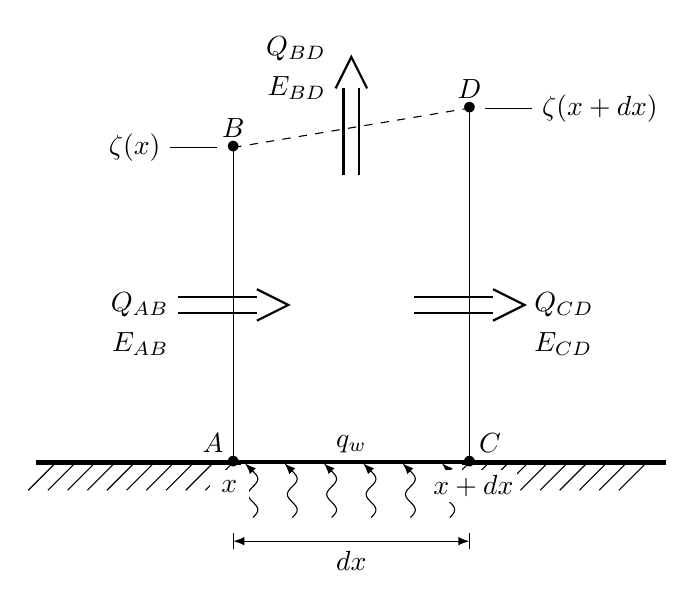
\begin{tikzpicture}
  % Tracé des parois
  \draw [ultra thick] (-4,-1) -- (4,-1);
  \foreach \i in {0,..., 9,10,21,22,...,30}
  {
    \pgfmathsetmacro{\x}{(- 4 + \i/4)};
    \draw (\x+1/4,-1) -- ++(-135:0.5);
  }
  \draw (-1.5, -1) node {$\bullet$};
  \draw ( 1.5, -1) node {$\bullet$};
  \fill (-1.4, -1.025) [white] rectangle (1.4, -1.8);
  %Repères et autres flèches
  \foreach \i in {0,...,5}
  {
    \pgfmathsetmacro{\y}{(-1.25 + \i/2)};
    \draw [domain=0:3*pi] plot ({sin(deg(\x))/16 + \y}, {\x/16-1.7}) [>=latex, ->] -- ++(-0.1,0.1);
  }
  \draw (0, -1) node [above] {$q_w$};
  \fill (-1.8, -1.1) [white] rectangle (-1.3, -1.5);
  \draw (-1.55, -1.3) node {$x$};
  \fill (1 , -1.1) [white] rectangle (2.1, -1.5);
  \draw (1.55,-1.3) node {$x+dx$};

  \draw (-1.5, -1) node [above left] {$A$} -- (-1.5, 3) node {$\bullet$} node [above] {$B$};
  \draw (-1.5, 3) [dashed] -- (1.5, 3.5) node {$\bullet$} node [above] {$D$};
  \draw (1.5, 3.5) -- (1.5, -1) node [above right] {$C$};

  \draw (0.8, 0.9) [thick] -- (1.8, 0.9);
  \draw (0.8, 1.1) [thick] -- (1.8, 1.1);
  \draw (1.8, 0.8) [thick]-- (2.2, 1) -- (1.8, 1.2);

  \draw (-2.2, 0.9) [thick] -- (-1.2, 0.9);
  \draw (-2.2, 1.1) [thick] -- (-1.2, 1.1);
  \draw (-1.2, 0.8) [thick] -- (-0.8, 1) -- (-1.2, 1.2);

  \draw (-0.1, 2.65) [thick] -- (-0.1, 3.75);
  \draw (0.1, 2.65) [thick] -- (0.1, 3.75);
  \draw (-0.2, 3.75) [thick] -- (0, 4.15) -- (0.2, 3.75);

  \draw (-2.2, 1) node [left] {$Q_{AB}$};
  \draw (-2.2, 0.5) node [left] {$E_{AB}$};

  \draw (2.2, 1) node [right] {$Q_{CD}$};
  \draw (2.2, 0.5) node [right] {$E_{CD}$};

  \draw (-0.2, 3.75) node [left] {$E_{BD}$};
  \draw (-0.2, 4.25) node [left] {$Q_{BD}$};

  \draw (-1.7, 3) -- (-2.3, 3) node [left] {$\zeta(x)$};
  \draw (1.7, 3.5) -- (2.3, 3.5) node [right] {$\zeta(x + dx)$};

  \draw (-1.5, -2) [>=latex,<->]-- (1.5, -2);
  \draw (-1.5, -2.1) -- (-1.5, -1.9);
  \draw (1.5, -2.1) -- (1.5, -1.9);
  \draw (0, -2) node [below] {$dx$};

\end{tikzpicture}

      \caption{Approche intégrale de von Karman pour le transfert de chaleur: volume de contrôle différentiel}
      \label{fig:vonKarman}
    \end{figure}

    La conservation de l'énergie dit que
    \begin{equation}
      E_{CD} + E_{BD} - E_{AB} = E_{AC}
    \end{equation}

    Sous écoulements compressibles, en enthalpie totale, on a
    \begin{equation}
      \begin{aligned}
        E_{AB} &= \left(\int_0^\zeta \rho u H_0 dy\right)\eval_x,\\
        E_{CD} &= \left(\int_0^\zeta \rho u H_0 dy\right)\eval_{x+dx},\\
        &= \left(\int_0^\zeta \rho u H_0 dy\right)\eval_x + dx \dv{x}\left(\int_0^\zeta \rho u H_0 dy\right)\eval_x,\\
        E_{BD} &= H_0 Q_{BD} = -H_{0e} dx \dv{x}\left(\int_0^\zeta \rho u dy \right)\eval_x
      \end{aligned}
    \end{equation}
    L'apport reçu par le fluide provient de l'échange de chaleur à la paroi
    \begin{equation}
      E_{AC} = dx q_w \eval_x
    \end{equation}

    Finalement, on obtient l'équation
    \begin{equation}
      dx\dv{x} \left(\int_0^\zeta \rho u H_0 dy\right) \eval_x - H_{0e} dx \dv{x}\left(\int_0^\zeta \rho u dy \right) \eval_x = dx q_w \eval_x
    \end{equation}
    Pour tout $x$, on peut établir\footnote{$H_{0e}$ est conservé en dehors de la couche limite: $\dv{H_{0e}}{x} = 0$}
    \begin{equation}
      \dv{x}\left(\int_0^\zeta \rho u (H_0 - H_{0e})\right) = q_w
    \end{equation}

    L'épaisseur d'enthalpie totale $\theta_{H_0}$ est définie par
    \begin{equation}
      \begin{aligned}
        \theta_{H_0} = \int_0^\zeta \frac{\rho u}{\rho_e u_e} \left(1 - \frac{H_0 - H_w}{H_{0e} - H_w} \right) dy &= \int_0^\zeta \frac{\rho u}{\rho_e u_e} \frac{H_{0e} - H_0}{H_{0e} - H_w} ~dy\\
        &= \int_0^\zeta \frac{\rho u}{\rho_e u_e} \frac{H_0 - H_{0e}}{H_w - H_{0e}} ~dy
      \end{aligned}
    \end{equation}

    L'équation intégrale de l'énergie est donc
    \begin{equation}
      \dv{x} (\rho_e u_e (H_w - H_{0e}) \theta_{H_0}) = q_w
    \end{equation}
    ou, en forme adimensionnelle
    \begin{equation}
      \dv{\theta_{H_0}}{x} + \left(\recip{\rho_e} \dv{\rho_e}{x} + \recip{u_e} \dv{u_e}{x} + \recip{H_w - H_{0e}} \dv{H_w}{x}\right) \theta_{H_0} = \frac{q_w}{\rho_e u_e (H_w - H_{0e}}) = St
    \end{equation}

    Dans le cas incompressible, on a $\rho = \rho_e$ invariable et on utilise l'énergie totale $U_0 = U + u^2/2$ à la place de l'enthalpie. On a alors
    \begin{equation}
      \theta_{U_0} = \int_0^\zeta \frac{u}{u_e}\left(1 - \frac{U_0 - U_w}{U_{0e} - U_w}\right) dy = \int_0^\zeta \frac{u}{u_e} \frac{U_0 - U_{0e}}{U_w ) U_{0e}} ~dy
    \end{equation}
    On obtient donc les équations intégrale et intégrale adimensionnelle
    \begin{align}
      \rho \dv{x} (u_e (U_w - U_{0e})\theta_{H_0}) &= q_w,\\
      \dv{\theta_{H_0}}{x} + \left(\recip{u_e} \dv{u_e}{x} + \recip{U_w - U_{0e}}\dv{U_w}{x}\right) \theta_{U_0} &= \frac{q_w}{\rho u_e (U_w - U_{0e})} = St
    \end{align}
